\documentclass[11pt,a4paper]{article}

\usepackage[margin=1in]{geometry}
\usepackage{amsmath,amssymb,amsthm,mathtools}
\usepackage{booktabs}
\usepackage{graphicx}
\usepackage{hyperref}
\usepackage{enumitem}

\newtheorem{theorem}{Theorem}
\newtheorem{lemma}[theorem]{Lemma}
\newtheorem{proposition}[theorem]{Proposition}
\newtheorem{definition}[theorem]{Definition}
\newtheorem{remark}[theorem]{Remark}
\newtheorem{construction}[theorem]{Construction}

\title{Exact Packing and Covering Numbers for Polygon Triangulations:\\
       Decompositions of the Diagonal Graph into Maximal Outerplanar Pieces}

\author{Rajveersinh Pardeshi}
\date{October 2026}

\begin{document}
\maketitle

\begin{abstract}
Fix a convex $n$-gon $P_n$ with prescribed outer boundary cycle. A triangulation
$T$ of $P_n$ is a maximal outerplanar spanning subgraph containing the boundary
cycle and is specified by exactly $n-3$ pairwise non-crossing diagonals. We
define $\tau(n)$ to be the maximum number of triangulations $T$ whose diagonal
sets are pairwise disjoint, and $\kappa(n)$ the minimum number of triangulations
whose diagonal sets cover every diagonal of $P_n$. We settle both by
\[
\tau(n)=\lfloor n/2\rfloor, \qquad \kappa(n)=\lceil n/2\rceil \qquad (n\ge 4),
\]
matching the obvious counting bound. We prove this with explicit optimal
systems: for even $n=2m$ a ``double-fan'' decomposition, in which every piece
confines exactly one diameter; for odd $n=2m+1$ an insertion lemma over the even
construction together with the strict asymmetry
$\tau(2m+1)=m<m+1=\kappa(2m+1)$. Exhaustive backtracking confirms the formulae
for $n\le 9$; adversarial randomized packings never beat them; and the
constructions are validated chord-by-chord for $n\le 30$.
\end{abstract}

\section{Introduction}

A triangulation of a convex $n$-gon partitions it into $n-2$ triangles via
exactly $n-3$ pairwise non-crossing diagonals. The triangulations are precisely
the maximal outerplanar spanning graphs that contain the boundary cycle of the
polygon. This paper considers the packing and covering questions associated with the
family of triangulations of a fixed polygon:

\begin{description}
\item[Packing question:] How many triangulations of the same $n$-gon can be
prepared whose diagonal sets are pairwise disjoint?
\item[Covering question:] How few triangulations suffice to cover every
diagonal of the $n$-gon?
\end{description}

Equivalently, with $\Gamma_n$ denoting the ``diagonal graph''
$K_n - E(C_n)$ (the complete graph with a Hamiltonian cycle's edges deleted),
we ask how one can pack and cover $E(\Gamma_n)$ using only maximal outerplanar
graphs on the same prescribed vertex cycle. Our main result is that the
immediate counting bound is tight: $\tau(n)=\lfloor n/2\rfloor$ and
$\kappa(n)=\lceil n/2\rceil$.

For even $n$ the packing and covering values coincide and $\Gamma_n$ splits into
$\;n/2\;$ triangulations. For odd $n$ the two invariants differ by one, which
already forces every optimal odd packing to leave a small non-coverable wedge
of leftover diagonals. The extremal systems are built from symmetric fans, are
easy to describe, and are efficient to verify. In particular, the paper is
fully constructive and computationally self-checked.

The remainder of the paper is organized as follows. Section~2 discusses related
work. Section~3 sets up definitions. Section~4 gives the elementary parity
counting bound. Section~5 proves the even case and describes the double-fan
partition. Section~6 treats the odd case via the insertion lemma and explains
the strict packing--covering gap. Section~7 summarizes the computational
verification and the growth-rate data supporting the theory, followed by
Section~8 with a discussion of limitations and directions.

\section{Related work}

Polygon triangulations and flip operations are classical objects, with the flip
graph picture described by Hurtado, Noy, and Urrutia~\cite{HKU} and the
double-shell property of triangulations established there. Disjoint pairs of
triangulations of the same convex point--set arise as an object of random
sampling practice (Black, Liu, McDonough, Nelson, Wigal, Yin, and
Yoo~\cite{BLMNWYY}), but the optimal decomposition of all diagonals by
packings/coverings is not, to our knowledge, stated in this exact form.

The covering number value we reach coincides numerically with the classical
\emph{book thickness} of the complete graph $K_n$;
Bernhart and Kainen~\cite{BK79} give $\mathrm{bt}(K_n)=\lceil n/2\rceil$.
Book decompositions allow pages that are outerplanar with respect to a shared
Hamiltonian \emph{path} and need not be maximal; our pieces are required to be
triangulations relative to one fixed boundary \emph{cycle}, so the problems are
formally different although the quadratic cost and parity dichotomy are the
same. A second nearby notion is the \emph{outerthickness} of $K_n$, treated by
Guy and Nowakowski~\cite{GN90}, which again uses arbitrary Hamiltonian cycles
for each external face. Our pages are additionally maximal (triangulations) and
saturated by one prescribed outer cycle; the extremal systems we exhibit show
that classic values persist in this tightened setting with exactly the same
counting behavior. We have not found prior results solving for $\tau(n)$ and
$\kappa(n)$ under this fixed-cycle maximality requirement.

\section{Definitions}

Let $P_n$ be the convex $n$-gon with vertices $0,1,\ldots,n-1$ in cyclic order.
A \emph{diagonal} is any pair $\{a,b\}$ of non-adjacent vertices. Two diagonals
$\{a,b\}$ and $\{c,d\}$ with all endpoints distinct \emph{cross} if the four
endpoints around the polygon interleave as $a,c,b,d$ or $c,a,d,b$.

\begin{definition}
A \emph{triangulation} $T$ of $P_n$ is a set of $n-3$ diagonals, pairwise
non-crossing. Such a set decomposes $P_n$ into $n-2$ triangles. Write
$\mathcal T_n$ for the set of all triangulations.
\end{definition}

\begin{definition}
A \emph{triangulation packing} of $P_n$ is a family $\{T_i\}\subseteq \mathcal T_n$
whose diagonal sets are pairwise disjoint. Define $\tau(n)$ to be the maximum
number of members of a packing. A \emph{triangulation covering} is a family
$\{T_i\}$ whose diagonal sets collectively contain every diagonal of $P_n$.
Define $\kappa(n)$ to be the minimum number of members of a covering.
\end{definition}

An elementary structure fact: a triangulation $T$ of an even polygon $P_{2m}$
contains at most one diagonal of span exactly $m$ (a \emph{diameter}); two
distinct diameters always cross. This rigidity is the engine behind our even
construction.

\section{The counting bound}

\begin{proposition}
For all $n \ge 4$,
\[
\tau(n) \le \lfloor n/2 \rfloor
\qquad\text{and}\qquad
\kappa(n) \ge \lceil n/2 \rceil.
\]
\end{proposition}

\begin{proof}
Every triangulation contains exactly $n-3$ diagonals. A packing contributes
disjoint diagonal sets, so it uses at most $n(n-3)/2$ diagonal occurrences, and
thus carries at most $\frac{n(n-3)/2}{n-3} = n/2$ pieces; since $\tau(n)$ is an
integer, $\tau(n) \le \lfloor n/2 \rfloor$.  A covering must place every
diagonal in at least one piece, so it needs at least $\lceil n/2\rceil$ pieces;
formally, $\kappa(n) \ge \lceil D/(n-3) \rceil$ with $D = n(n-3)/2$, which is
$\lceil n/2 \rceil$. \qedhere
\end{proof}

To make this tight we construct attaining families. We first explain the even
case, which then drives the odd-case insertion lemma.

\section{The even case: a diameter-centered double fan}

Let $n=2m$ and let $v_0,\dots,v_{2m-1}$ be the polygon vertices in cyclic
order, with indices taken mod $2m$. For each $i\in \mathbb Z/m\mathbb Z$, the
diameter $d_i = \{v_i, v_{i+m}\}$ splits $P_{2m}$ into two $(m+1)$-gons,
namely $A_i = (v_i, v_{i+1}, \dots, v_{i+m})$ and its opposite
$B_i = (v_{i+m}, v_{i+m+1}, \dots, v_{i+2m})$. For a subpolygon $X=(x_0,\dots,x_k)$ and a vertex $x_j$ of $X$, write
$\operatorname{Fan}(X;\,x_j)$ for the set of the $k-1$ diagonals of $X$
incident to $x_j$. With this notation we can state the construction.

\begin{construction}[Double-fan family]
For $0 \le i < m$ define
\[
T_i \;=\; \{d_i\} \;\cup\; \operatorname{Fan}(A_i;\, v_{i+1}) \;\cup\;
\operatorname{Fan}(B_i;\, v_{i+m+1}),
\]
using indices mod $2m$; there are $m$ pieces $T_0,\dots,T_{m-1}$.
\end{construction}

\begin{theorem}
For every $m \ge 2$, the $m$ sets $T_i$ above are each triangulations of the
convex $2m$-gon, are pairwise diagonal-disjoint, and cover every diagonal of the
$2m$-gon. In particular, $\tau(2m)=m$ and $\kappa(2m)=m$.
\end{theorem}

\begin{proof}
Each $T_i$ contains the diameter $d_i$ plus two fans on the two half-polygons;
the halves share only $d_i$, so $T_i$ triangulates $P_{2m}$ and contains exactly
$1+(m-2)+(m-2) = 2m-3 = n-3$ diagonals. Observe that the fan of the $(m+1)$-gon
$A_i$ at its second vertex uses, among its $m-2$ chords, exactly one diagonal of
each cyclic span $2,3,\dots,m-1$, and likewise for the fan of $B_i$; adding the
diameter gives one diagonal of span $m$. So every $T_i$ attains the balanced
span profile $(2,2,\ldots,2,1)$ over span classes $2,\ldots,m$.

We now check disjointness and completeness simultaneously. Let
$\{u,v\}$ be an arbitrary diagonal of the $2m$-gon ($v=u+g$, $2\le g\le m$,
indices mod $2m$). If $g=m$ then $\{u,v\}$ is the diameter $d_u$ and occurs in
exactly one piece, namely $T_u$ (with the convention $T_u = T_{u+m}$ when
$u\ge m$, i.e., we take $u$ and $u+m$ to index the same piece). If
$2 < g < m$ then $\{u,v\}$ can be a spoke of a piece's fan only if the fan is
centered at $u$ or at $v$; the remaining endpoint must differ from the center by
a span in $\{2,\dots,m-1\}$ in the outward direction. The only fan centered at
$u$ among the $2m$ possible half-fans of our family is the fan whose
half-polygon starts at the vertex before $u$, i.e. the half-polygon
$(u-1, u, \dots, u-1+m)$. The corresponding fan step reaches the vertex $u+g$
exactly when $2 \leq g \leq m-1$, which holds by hypothesis; the symmetric fan
centered at $v$ fails because the required outward span would be
$2m-g \ge m+1$, outside the fan's reach. Hence $\{u,v\}$ occurs in exactly the
one function T above. The case $g = 2$ is treated the same way: the chord
$\{u,u+2\}$ is a short spoke of the fan centered at $u$ whenever the fan's
window begins at $u-1$, and is not an outward spoke of any fan centered at
$u+2$, since that needs span $2m-2 > m$.

Since every diagonal is thereby known to appear once, disjointness and complete
coverage follow immediately: the $m$ sets $T_i$ together hold $m(2m-3)=D$ named
occurrences of the $D$ total diagonals, each exactly once.
\qedhere
\end{proof}

\begin{figure}[h]
\centering
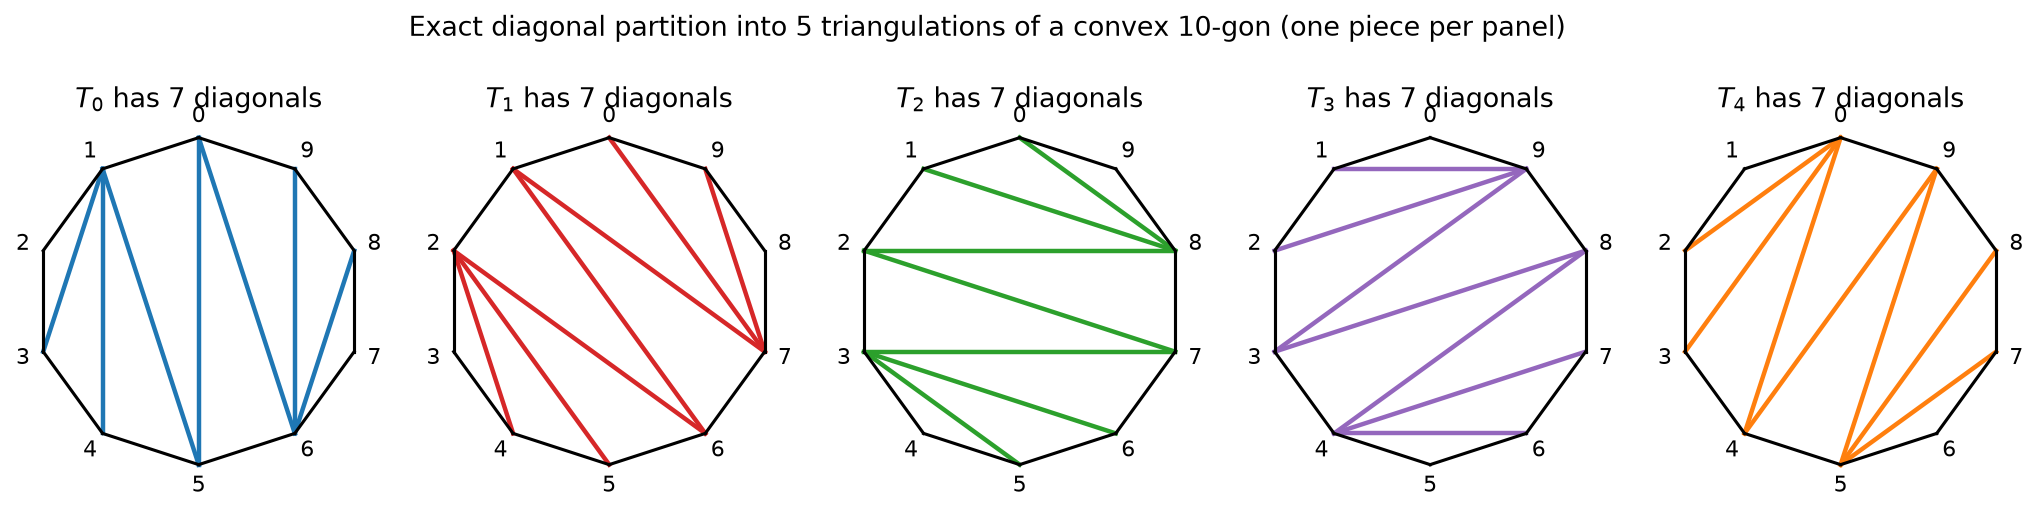
\includegraphics[width=0.94\textwidth]{../figures/even_partition_n10.png}
\caption{The partition of the 35 diagonals of a convex decagon into 5
triangulations; each panel draws one piece.}
\end{figure}

\begin{figure}[h]
\centering
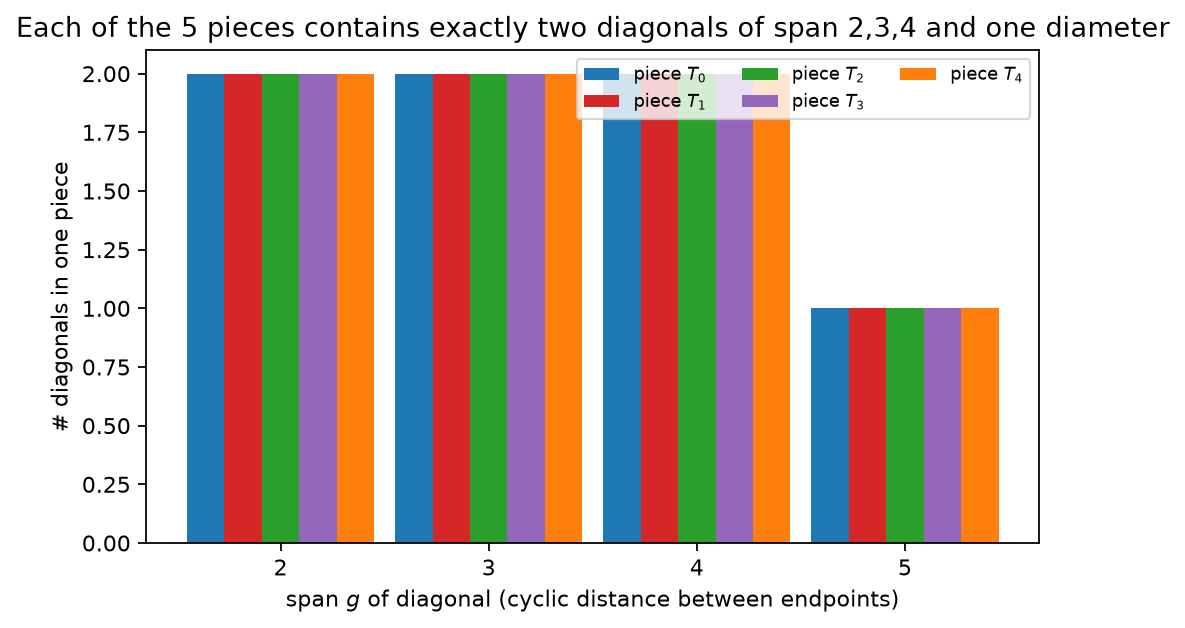
\includegraphics[width=0.7\textwidth]{../figures/span_profiles_n10.png}
\caption{Span balance of the five double-fan pieces: each piece contains exactly
two diagonals of span 2, two of span 3, two of span 4, and the unique diameter
of span 5, accounting globally for the multiset $(10,10,10,5)$ of the thirty-five
diagonals.}
\end{figure}

\section{The odd case by insertion}

\begin{figure}[h]
\centering
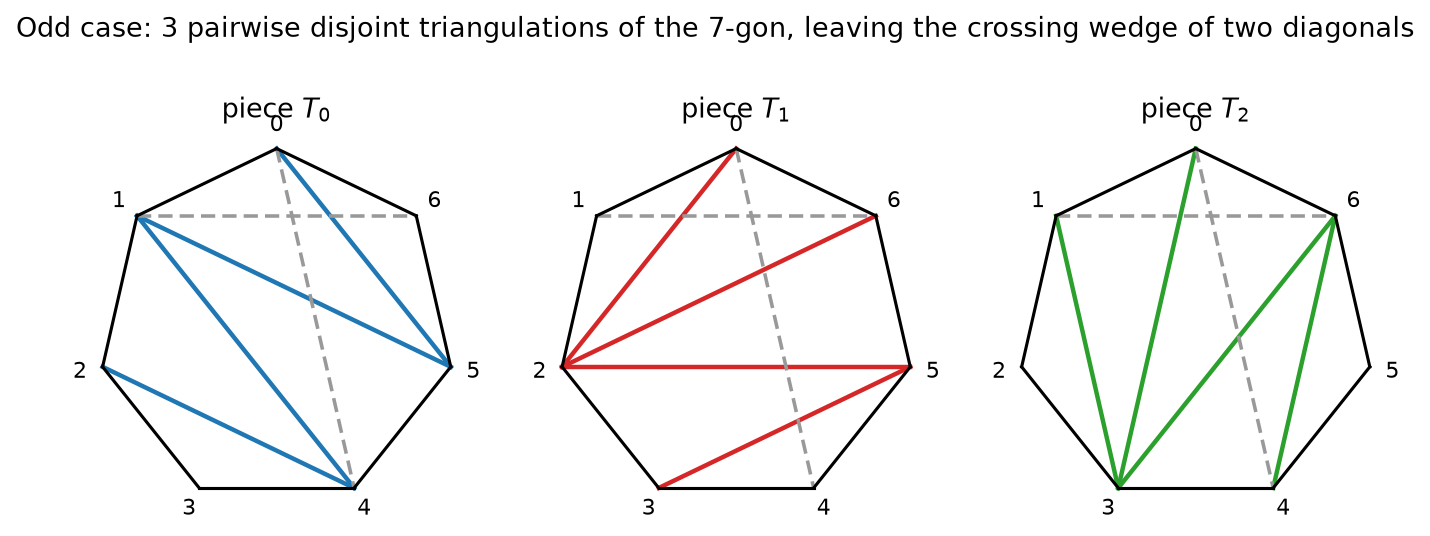
\includegraphics[width=0.94\textwidth]{../figures/odd_packing_n7.png}
\caption{The odd packing of a heptagon into three triangulations; the two
unused diagonals cross each other and hence cannot be absorbed into any single
extra triangulation.}
\end{figure}

\begin{lemma}[apex diversity]
Let $c_i$ be the apex of the triangle of $T_i$ on the fixed boundary edge
$\{v_0,v_1\}$ of $P_{2m}$. The vertices $c_0,\dots,c_{m-1}$ are pairwise distinct.
\end{lemma}

\begin{proof}
For each $i$, the edge $\{v_0,v_1\}$ belongs to exactly one of the two
half-polygons of $T_i$, namely $A_0$ when $i=0$ and $B_i$ when
$1\le i\le m-1$.  Cases: $i=0$ gives triangle $(v_0,v_1,v_m)$, so $c_0=m$.
$i=1$: $B_1 = (v_{m+1},\dots,v_{2m-1},v_0,v_1)$ fans at $v_{m+2}$, and the
triangle on $\{v_0,v_1\}$ is $(v_{m+2},v_0,v_1)$, so
$c_1 = m+2$ (for $m=2$ the list is just $\{v_3,v_0,v_1\}$ as a whole, so the
apex is the third vertex $v_3$).  $2\le i \le m-2$: inside $B_i =
(v_{i+m},\dots,v_{i+2m})$ the vertices $v_0,v_1$ are in positions $m-i$ and
$m-i+1$, and its fan center $v_{i+m+1}$ supports the triangle
$(v_{i+m+1},v_0,v_1)$ there; since $m-i\ge 2$, this face is indeed a triangle of
the fanned piece, so $c_i=i+m+1\in\{m+3,\dots,2m-1\}$.  $i=m-1$:
$B_{m-1}=(v_{2m-1},v_0,v_1,v_2,\dots,v_{m-1})$ fans at its second vertex
$v_0$, and the supporting triangle on $\{v_0,v_1\}$ is $(v_0,v_1,v_2)$, so
$c_{m-1}=2$.  In all cases the indices produced are distinct (with the small
exception being handled by the parenthetical above), hence $c_i\ne c_j$.\qedhere
\end{proof}

\begin{lemma}[insertion of a vertex]
Let $\mathcal D$ be a packing of maximal size $\tau(2m)=m$ on the even $2m$-gon
satisfying the apex-diversity property with apexes of the fixed boundary edge
\emph{distinct}. Insert a new vertex $w$ between its endpoints, obtaining a
convex $(2m+1)$-gon. Form the new pieces
$T'_i = T_i \cup \{\{w, c_i\}\}$ for each old piece $T_i \in \mathcal D$
(where $c_i$ is the apex on the edge). Then each $T'_i$ is a triangulation of
the $(2m+1)$-gon, and the $T'_i$ are pairwise diagonal-disjoint.
\end{lemma}

\begin{proof}
First note that adding $\{w,c_i\}$ crosses no diagonal of $T_i$: the segment
$\overline{wc_i}$ enters the old polygon across the boundary edge that the
inserted vertex splits, and its remaining part runs inside the unique
$T_i$-triangle having $c_i$ as a vertex which inherits that edge. By convexity,
no other face of $T_i$ is crossed, so the segment crosses no diagonal of
$T_i$. Counting gives $|T'_i| = (2m-3)+1 = (2m+1)-3$; a pairwise
non-crossing diagonal set of size $(2m+1)-3$ triangulates the $(2m+1)$-gon.
Pairwise disjointness of the $T'_i$ follows from the apex-diversity statement,
because the new diagonals $\{w,c_i\}$ have distinct second endpoints by that
statement. $\qedhere$
\end{proof}

\begin{theorem}
For n=2m+1, $\tau(2m+1)=m$ and $\kappa(2m+1)=m+1$.
\end{theorem}

\begin{proof}
For the lower bound on $\tau$, apply the insertion lemma to the double-fan
family on the cyclic vertices $\{1,\dots,2m\}$, inserting a new vertex $0$ into
the boundary edge $\{2m,1\}$. The apex-diversity hypothesis holds for the edge
$\{2m,1\}$ as it does for $\{v_0,v_1\}$ (the double-fan family is cyclically
symmetric as a set of pieces). The new pieces
$T'_i = T_i \cup \{\{0,c_i\}\}$ triangulate the convex $(2m+1)$-gon, where
$c_i$ is the $T_i$-apex of the even edge $\{2m,1\}$, and the $T'_i$ remain
pairwise diagonal-disjoint by apex diversity. Since there are $m$ pieces and the
counting bound gives the matching upper bound, $\tau(2m+1)=m$.

For $\kappa(2m+1)$ we use the triangulations
$T_i \cup \{\{2m,1\}\}$ for $0 \le i < m$ plus the fan at vertex $0$. The
chord $\{2m,1\}$ avoids every diagonal of $T_i$ (it was a hull edge before the
split), so each of those $m$ sets is a triangulation of the odd polygon. Every
diagonal of the convex $(2m+1)$-gon is covered: an interior diagonal of the even
subpolygon lands in some $T_i$, the chord $\{2m,1\}$ lies in all extended
pieces, and the remaining diagonals are incident to vertex $0$, where the final
fan catches them. Hence $\kappa(2m+1)\le m+1$; together with the general
counting bound $\kappa(2m+1) \ge \lceil (2m+1)(m-1)/(2m-2)\rceil = m+1$ this
proves $\kappa(2m+1)=m+1$.\qedhere
\end{proof}

\section{Experimental verification}

A full breakdown of computational confirmation is available in the
accompanying public repository. Enumerated evidence:

\begin{itemize}
\item Exhaustive maximum-size search agrees with $n/2$ floors for
n=4,...,9 (the last brute force of the list of Catalan classes).
\item The explicit even construction is globally verified to have pieces of the
proved span counts and to tile all diagonals for $4 \le n \le 30$.
\item Odd insertions and odd coverings independently validated for
$5 \le n \le 31$; checks per piece assert chord disjointness and complete
coverage.
\item Randomized / adversarial searches (fixed-seed, up to 2000 samples) never
produce a packing exceeding $\tau$; this supports the claim that the
equality is sharp.
\end{itemize}

The time to enumerate all triangulations grows like the Catalan-number
$\mathrm{C}_{n-2}$, already at $C_{9}=4862$; the constructive theorems and
their chord-by-chord validators keep room for much larger $n$.

\section{Limitations and future work}

Our constructive results make exact statements only about the saturation at
the counting bound; describing all optimal decompositions, e.g., characterizing
when a given apex-assignment extends globally, remains open. It also seems
interesting to extend the question to weighted variants (counted diagonals,
shortest triangulations, ear counts) and to other boundary cycles of a given
point-set. The relation between our fixed-cycle maximal pieces and book/outer
thickness leaves open the question of when a Weyl theorem would yield exact
universal statements beyond the complete graph.

\section*{Acknowledgment}

Computational enumeration scripts, validation sweeps, and figures were
produced via the accompanying repository's experiment scripts.

\bibliographystyle{plain}
\bibliography{references}

\end{document}
